\section{Results}
\label{sec:results}

Clean recall is 0.745--0.792 on HERIDAL and 0.879--0.891 on SARD,
consistent with SARD's lower-altitude capture and larger relative object
size. Every number reported below is recall at that model's own frozen
operating point unless stated otherwise, and every condition carries a
bootstrap interval in the released per-condition table.

\subsection{Degradation is uneven and does not transfer}

At matched severity 3 on SARD, YOLOv11 recall ranges from 0.855 under
\cfd{rain\_streaks}, a 3.6-point drop from its 0.891 clean baseline, to
exactly 0.000 under \cfd{low\_light} (Table~\ref{tab:spectrum}). That is
the whole span of the outcome space inside one dataset, one model and
one severity level, which is the first reason a single averaged
robustness score is the wrong summary for this task.

The same corruption also behaves differently across capture regimes.
\cfd{rain\_streaks} is the mildest corruption on SARD for all three
detectors, yet on HERIDAL it sits among the most damaging, where the
storm-family relative recall drop reaches 0.784--0.874. We do not
isolate which property of the capture regime produces the reversal, and
the obvious candidate is not straightforward: by COCO area bands both
test sets are dominated by medium-sized instances (327 of 337 on
HERIDAL, 789 of 1097 on SARD), so absolute subject size alone does not
explain it. What the result does establish is the consequence: a
robustness number measured at one altitude does not transfer to another,
which matters directly for anyone selecting a system against a mission
profile.

Table~\ref{tab:family} aggregates relative recall drop by disaster
family across all three detectors and both datasets. Flood is the
mildest family without exception, the one ordering fully consistent
across the study. Storm is worst on HERIDAL, pulled up by the low-light
collapse, and earthquake is worst on SARD. Figure~\ref{fig:heatmap}
shows the same pattern per corruption, with the \cfd{low\_light} row
saturating for all three architectures.

\begin{table}[t]
\centering\small
\setlength{\tabcolsep}{3pt}
\caption{Mean relative recall drop by disaster family, averaged over
severities. Flood is mildest on both datasets for every model; storm is
worst on HERIDAL, earthquake worst on SARD.}
\label{tab:family}
\begin{tabular}{lccc}
\toprule
Family & F.\ R-CNN & RT-DETR & YOLOv11 \\
\midrule
\multicolumn{4}{l}{\emph{HERIDAL}} \\
Storm      & 0.784 & 0.874 & 0.829 \\
Earthquake & 0.534 & 0.568 & 0.571 \\
Wildfire   & 0.335 & 0.459 & 0.405 \\
Flood      & 0.301 & 0.231 & 0.246 \\
\midrule
\multicolumn{4}{l}{\emph{SARD}} \\
Earthquake & 0.481 & 0.630 & 0.624 \\
Storm      & 0.401 & 0.440 & 0.413 \\
Wildfire   & 0.327 & 0.451 & 0.445 \\
Flood      & 0.264 & 0.293 & 0.252 \\
\bottomrule
\end{tabular}
\end{table}

\begin{figure}[t]
\centering
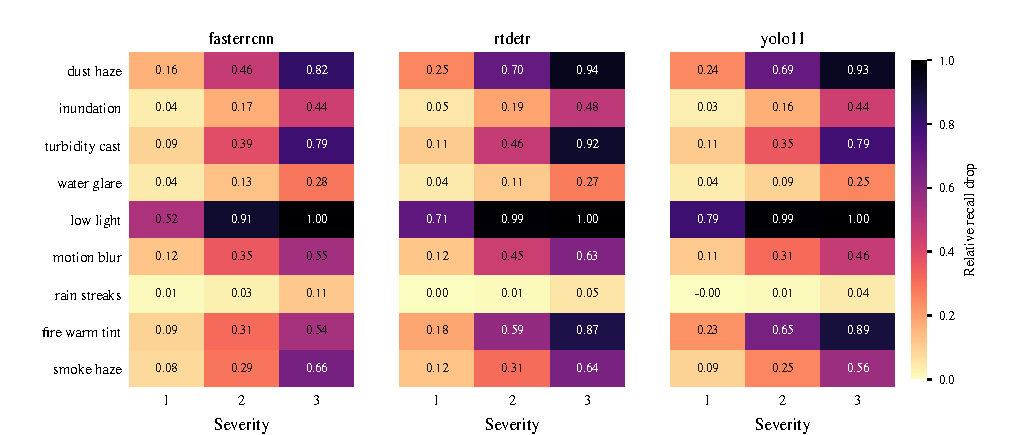
\includegraphics[width=\columnwidth]{figures/heatmap_sard.pdf}
\caption{Relative recall drop, (clean$-$corrupted)/clean, for each
detector on SARD. Rows grouped by disaster family. The
\cfd{low\_light} row saturates for all three architectures.}
\label{fig:heatmap}
\end{figure}

\subsection{Low light collapses detection across all architectures}

By severity 3, recall is exactly 0.000 for all three architectures on
both HERIDAL ($n{=}101$ images, 337 persons) and SARD ($n{=}862$ images,
1097 persons), and every one of 1000 bootstrap resamples agrees, so the
interval is degenerate at $[0.000,0.000]$ (Table~\ref{tab:lowlight}).
Not one annotated person is recovered anywhere in either test set. A
two-stage CNN, a single-stage CNN and a transformer sit at the same
floor, which rules out an architecture-specific explanation, and the
condition producing it is an exposure loss of about 4.5 stops rather
than true darkness.

\paragraph{It is not the threshold.} The natural objection is that a
frozen-threshold zero reflects a badly placed operating point rather
than a failure to detect. mAP$_{50}$ settles it, since it scans every
threshold: on HERIDAL at severity~1, RT-DETR's mAP$_{50}$ falls from
0.835 clean to 0.001, YOLOv11's from 0.803 to 0.064 and Faster R-CNN's
from 0.785 to 0.537, in lockstep with frozen-threshold recall. Were this
a calibration artefact, mAP would stay high while recall fell; it does
not. The same point holds across models rather than only within one:
Faster R-CNN is consistently the most robust wherever any model retains
recall, despite carrying the strictest frozen threshold (0.99 on
HERIDAL, 0.96 on SARD), which rules out threshold strictness as the
explanation for the ordering.

\paragraph{It is not the seed.} A single training run per model leaves
open that the zero is a property of one unlucky checkpoint. We repeated
the SARD YOLOv11 run at two further seeds, 42 and 123, each trained and
threshold-selected independently under the identical protocol, and
re-swept the low-light ladder (Table~\ref{tab:seeds}). Clean recall
moves only between 0.874 and 0.891 and the independently selected
threshold moves only between 0.30 and 0.35, so the three runs are
comparable. Severity-1 recall varies materially, from 0.184 to 0.234,
which is worth noting as the honest scale of run-to-run variation on
this ladder. Severity 3 does not vary at all: all three seeds return
exactly 0.000 with degenerate intervals. The collapse is a property of
the condition, not of a checkpoint.

\begin{table}[t]
\centering\small
\setlength{\tabcolsep}{3.5pt}
\caption{Multi-seed repeat, YOLOv11 on SARD, under \cfd{low\_light}.
Each seed is trained and threshold-selected independently. Bootstrap
95\% intervals over 1000 resamples in brackets. Severity-1 recall varies
across seeds; severity 3 is exactly zero for all three.}
\label{tab:seeds}
\begin{tabular}{lccc}
\toprule
 & Seed 17 & Seed 42 & Seed 123 \\
\midrule
Threshold & 0.30 & 0.35 & 0.30 \\
Clean     & 0.891 & 0.874 & 0.885 \\
\midrule
s1 & 0.184 & 0.200 & 0.234 \\
   & \ci{0.154}{0.213} & \ci{0.170}{0.229} & \ci{0.207}{0.265} \\
s2 & 0.007 & 0.008 & 0.021 \\
   & \ci{0.003}{0.013} & \ci{0.003}{0.014} & \ci{0.012}{0.029} \\
s3 & \textbf{0.000} & \textbf{0.000} & \textbf{0.000} \\
   & \ci{0.000}{0.000} & \ci{0.000}{0.000} & \ci{0.000}{0.000} \\
\bottomrule
\end{tabular}
\end{table}

\paragraph{It is not only the corruption model.} Because the corruption
is synthetic, we evaluated the SARD-trained YOLOv11, at its frozen
operating point and without retraining, on 40 real nighttime images from
VisDrone~\cite{zhu2022visdrone}, held out from training, calibration and
threshold selection. Recall was 0.016, close to the floor the synthetic
corruption reaches at severity 3. The settings are not equivalent, as
VisDrone night scenes are urban and artificially lit whereas
search-and-rescue imagery is unlit terrain, and 40 images is a spot
check rather than a benchmark. Read narrowly, it indicates the failure
is not an artefact of the corruption model. We state the weakness of
this check plainly in Section~\ref{sec:discussion} rather than resting
the claim on it.

Taken together, the three checks close off the three ways this result
could have been an artefact of our own setup. What remains is a property
of photon-limited aerial imagery and the detectors as trained.

\subsection{The failure is a loss of detections, not of localisation}

For instances detected in both the clean and corrupted conditions, we
measure the IoU between the two predicted boxes, a scale-normalised
centre shift, and the drop in box-versus-ground-truth fit. Restricting
to commonly detected instances keeps the metric unconfounded by recall:
it asks whether a surviving detection stayed planted on the person,
which is a different question from whether the person was found at all.

Figure~\ref{fig:decoupling} plots recall against localisation stability
for YOLOv11 on SARD, one point per corruption and severity, with both
axes spanning the full unit range. Stability declines only from 0.98 to
0.78 across the entire severity range while recall falls from 0.89 to
0.00, and the count of commonly detected instances tracks recall exactly
(\cfd{low\_light}: 202, then 8, then 0). Recall sweeps nearly the whole
unit range while stability stays in a narrow band near the top, never
below 0.78 even where almost every detection is lost.

The dominant failure mode is therefore a detection disappearing, not a
box drifting off the person. This matters operationally: a mislocalised
box is a visible error an operator can catch, whereas a frame with no
detections is indistinguishable from a correctly searched empty frame.
Under the conditions measured here, these systems fail silently, in the
direction that resembles task completion. It also says where a
mitigation should aim, at sensitivity rather than at localisation, which
is the design the next section tests.

\begin{figure}[t]
\centering
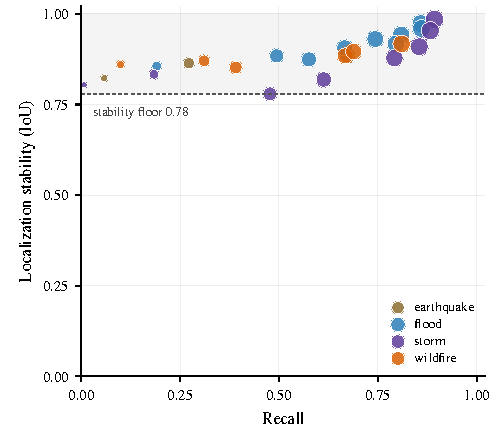
\includegraphics[width=0.85\columnwidth]{figures/decoupling_sard_yolo11.pdf}
\caption{Recall against localisation stability, YOLOv11 on SARD, one
point per corruption and severity. Points sweep the entire recall range
while remaining in a narrow band near the top of the stability axis.}
\label{fig:decoupling}
\end{figure}

\begin{table}[t]
\centering\small
\setlength{\tabcolsep}{4pt}
\caption{Recall by corruption and severity, YOLOv11 on SARD, at the
frozen operating point of 0.30. Clean baseline 0.891. The span within
this single table, 0.855 to 0.000 at severity 3, is why an averaged
robustness score is the wrong summary.}
\label{tab:spectrum}
\begin{tabular}{llccc}
\toprule
Corruption & Family & s1 & s2 & s3 \\
\midrule
\cfd{rain\_streaks}    & Storm      & 0.893 & 0.882 & \textbf{0.855} \\
\cfd{water\_glare}     & Flood      & 0.859 & 0.809 & 0.666 \\
\cfd{inundation}       & Flood      & 0.861 & 0.744 & 0.495 \\
\cfd{motion\_blur}     & Storm      & 0.792 & 0.613 & 0.478 \\
\cfd{smoke\_haze}      & Wildfire   & 0.810 & 0.667 & 0.391 \\
\cfd{turbidity\_cast}  & Flood      & 0.796 & 0.575 & 0.191 \\
\cfd{fire\_warm\_tint} & Wildfire   & 0.688 & 0.310 & 0.099 \\
\cfd{dust\_haze}       & Earthquake & 0.674 & 0.273 & 0.058 \\
\cfd{low\_light}       & Storm      & 0.184 & 0.007 & \textbf{0.000} \\
\bottomrule
\end{tabular}
\end{table}

\begin{table}[t]
\centering\small
\setlength{\tabcolsep}{3pt}
\caption{Recall under \cfd{low\_light} at each model's frozen operating
point, with clean recall for reference. Once recall is exactly zero on
the full test set every bootstrap resample returns zero, so the interval
is degenerate by construction.}
\label{tab:lowlight}
\begin{tabular}{lccccc}
\toprule
Model & Thr. & Clean & s1 & s2 & s3 \\
\midrule
\multicolumn{6}{l}{\emph{HERIDAL} (101 images, 337 persons)} \\
Faster R-CNN & 0.99 & 0.745 & 0.451 & 0.110 & \textbf{0.000} \\
YOLOv11      & 0.45 & 0.769 & 0.047 & 0.000 & \textbf{0.000} \\
RT-DETR      & 0.65 & 0.792 & 0.000 & 0.000 & \textbf{0.000} \\
\midrule
\multicolumn{6}{l}{\emph{SARD} (862 images, 1097 persons)} \\
Faster R-CNN & 0.96 & 0.879 & 0.419 & 0.077 & \textbf{0.000} \\
RT-DETR      & 0.60 & 0.888 & 0.260 & 0.013 & \textbf{0.000} \\
YOLOv11      & 0.30 & 0.891 & 0.184 & 0.007 & \textbf{0.000} \\
\bottomrule
\end{tabular}
\end{table}
